\section{Advice for Applying Machine Learning}

\subsection{Deciding What to Try Next}
    Potential next steps:
    \begin{enumerate}
        \item Larger training data.
        \item Smaller set of feature.
        \item Additional features.
        \item Polynomial features.
        \item Increase $\lambda$.
        \item Decrease $\lambda$. 
    \end{enumerate}

    Machine Learning Diagnostic: a test to run to gain insight on feasibility of techniques and how to optimize performance. 

\subsection{Evaluating Hypothesis: training/validation/test sets}
    \subsubsection{Motivation with Test sets}
    We want to address the problem of overfitting: fits training examples very well (low error) but fails to generalize and hence not inaccurate on additional data. Thus, to evaluate the true accuracy of hypothesis, we randomly split the data into two sets: a \textbf{training set} (70\%) and a \textbf{test set} (30\%). 
    The procedure :
    \begin{enumerate}
        \item Learn $\Theta$ and minimize $J_{train} (\Theta)$ using the training set
        \item Compute test set error: $J_{test} (\Theta)$. 
            \begin{enumerate}
                \item For linear regression: 
                    \[
                    J_{test} (\Theta) =  \frac{1}{2m_{test}} \sum_{i=1}^{m_{test}} (h_\theta(x_{test}^{(i)}) - y_{test}^{(i)} )^2
                    \]
                \item For logistic regression:
                    \[
                        J (\theta) = \frac{-1}{m_{test}} \sum_{i=1}^{m_{test}} (y^{(i)}_{test} log(h_{\Theta} ( x^{(i)}_{test}) + (1-y^{(i)}_{test}) log(1-h_{\Theta} ( x^{(i)}_{test}) )
                    \] 
                \item For classification, we first calculate the misclassification error. 
                    \begin{equation}
                        err (h_{\Theta} (x), y) = 
                        \begin{cases}
                            1 &\quad \text{if } (h_\Theta (x) \geq 0.5 \: \& \: y=0)\text{ or } (h_\Theta (x) \leq 0.5 \:\&\:  y=1) \\
                            0 &\quad \text{if otherwise. }  \\
                        \end{cases}
                        \label{eq:misclassification-error}
                    \end{equation}

                    The average test error is thus:
                    \begin{equation}
                        \text{Test error} = \frac{1}{m_{test}} \sum_{i=1}^{m_{test}} err (h_{\Theta} (x), y)
                        \label{eq:classification-test-error}
                    \end{equation}

            \end{enumerate}
    \end{enumerate}


    \subsubsection{Polynomial features: Train/Validation/Test model}
        \begin{itemize}
            \item Computed cost is less than the generalization error: We trained our data on the training set to obtain $\Theta$ with different degrees of polynomial (d). We then choose d based on minimizing the test set.
            \item Problem: $J_{test} (\Theta)$ is likely to be an optimistic generalization error, since the parameter d is fit to the test data set.
            \item Solution: break down dataset into three sections:
                \begin{enumerate}
                    \item Training set (60\%).
                    \item Cross-validation set (20\%).
                    \item Test set (20\%).
                \end{enumerate}

        \end{itemize}

        Procedure:
        \begin{enumerate}
            \item Optimize the parameters in $\Theta$ using the training set for each polynomial degree.
            \item Find the polynomial degree d with the least error using the cross validation set.
            \item Estimate the generalization error using the test set with $J_{test}(\Theta^{(d)})$, (d = theta from polynomial with lower error);
        \end{enumerate}

        This way, the degree of the polynomial d has not been trained using the test set.
    

    
        
\subsection{Diagnosing Bias vs Variance}
    \begin{itemize}
        \item Degree of polynomial (d) and underfitting (high bias) / overfitting (high variance).
        \item Training errors tend to decrease as d increases. 
        \item Cross validation error tends to form a convex curve with a minimum point. 
    \end{itemize}

    Therefore, the key to distinguish between bias and variance is summarized in Figure \ref{fig:error-bias-variance}. 
    \begin{figure}[htbp]
        \centering
        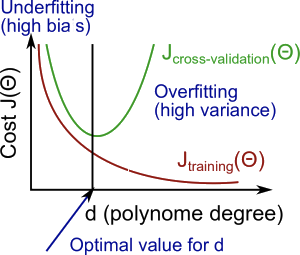
\includegraphics[width=0.5\textwidth]{image/error-bias-variance.png}
        \caption{Error cost of cross-validation and training over degree of polynomial}
        \label{fig:error-bias-variance}
    \end{figure}

    \begin{enumerate}
        \item \textbf{High bias (underfitting)}: both $J_{train} (\Theta)$ and $J_{CV} (\Theta)$ will be high. Thus: $J_{train} (\Theta) \approx J_{CV} (\Theta)$
        \item  \textbf{High variance (overfitting)}: \emph{Low} $J_{train} (\Theta)$ and \emph{high} $J_{CV} (\Theta)$. Thus: $J_{train} (\Theta) <<  J_{CV} (\Theta)$

    \end{enumerate}

\subsection{Regularization and bias and variance}
    \begin{itemize}
        \item Large $\lambda$ (lower significance of $\Theta$, heavy penalization so $h_\theta \approx 0$): high bias, underfit. 
        \item Small $\lambda$ (high significance of $\Theta$): high variance, overfit. 
    \end{itemize}

    Procedure to pick the right $\lambda$:
    \begin{enumerate}
        \item Create list of lambda. 
        \item Iterate through $\lambda$s and learn/obtain $\Theta$. 
        \item Compute cross-validation error ($J_{CV} (\Theta) $) using the learned $\Theta$ \textbf{without regularization} (i.e. $\lambda = 0$)
        \item Select the best lambda and Theta pair and verify on test set. (Compute $J_{test} (\Theta)$.
    \end{enumerate}
\subsection{Learning Curves}
    Plotting error over number of training examples. 
    \subsubsection{High bias}
        \begin{enumerate}
            \item Low training set size: low $J_{train}$ and high $J_{CV}$.
            \item Large training set size: high $J_{train}$ and high $J_{CV}$.
        \end{enumerate}

        Getting more training data will not help. 
        \begin{figure}[htbp]
            \centering
            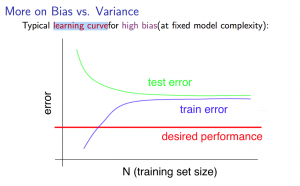
\includegraphics[width=\textwidth]{image/learning-curve-high-bias.png}
            \caption{Learning curve for high bias}
            \label{fig:learning-curve-high-bias}
        \end{figure}
    
    \subsubsection{High variance}
        \begin{enumerate}
            \item Low training set size: low $J_{train}$ and high $J_{CV}$.
            \item Large training set size: $J_{train}$ increases and $J_{CV}$ decreases.
        \end{enumerate}

        Getting more training data will help. 
        \begin{figure}[htbp]
            \centering
            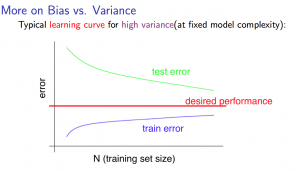
\includegraphics[width=\textwidth]{image/learning-curve-high-variance.png}
            \caption{Learning curve for high variance}
            \label{fig:learning-curve-high-variance}
        \end{figure}

\subsection{Summary}
    \begin{enumerate}
        \item Getting more training examples: Fixes high variance
        \item Trying smaller sets of features: Fixes high variance
        \item Adding features: Fixes high bias
        \item Adding polynomial features: Fixes high bias
        \item Decreasing $\lambda$: Fixes high bias
        \item Increasing $\lambda$: Fixes high variance.
    \end{enumerate}
\subsection {Neural Networks}
    \begin{enumerate}
        \item Small neural network: fewer parameters $\implies$ prone to underfitting, but computationally cheaper. 
        \item Large neural network: more parameters $\implies$ prone to overfitting, computationally expensive. Use regularization to address overfitting. 
    \end{enumerate}
    
